% included from comp for modification for possible inclusion
% ...  remake all LHCInfo plots with current incarnation .....

The LHC beams are composed of bunches of protons that are localized in buckets dictated by the RF cavity frequency. There are 35,640 buckets around the full circumference of the LHC but only a fraction of these buckets are filled with protons. There is a mandatory number of empty buckets required between every possibly filled bucket, called the abortion gap. The gap is necessary for the implementation of a beam dump. This requirement reduces the 35,640 possible buckets down to 2,808 allowed buckets.

\begin{figure}[htbp]
\begin{center}
\resizebox{0.7\linewidth}{!}{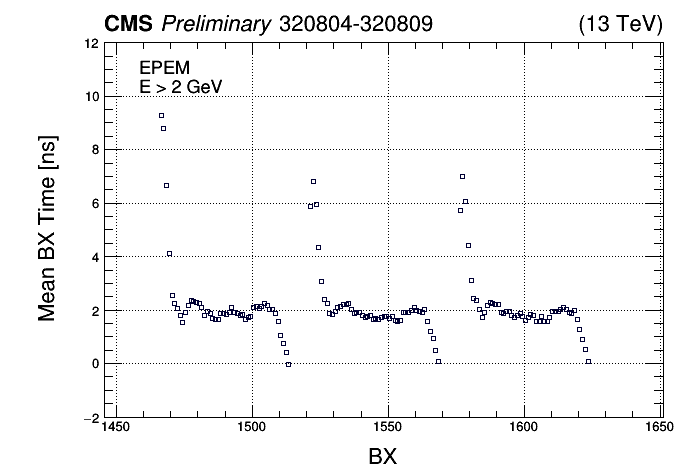
\includegraphics{fig/sec_motive/tr_lhc_18A_ratio2_note_05112021122552.png}}
\caption{The dependence of the rechit time on the position of a BX in a train of filled buckets. The mean of all the rechit times in a single BX are plotted with respect to the BX position of that BX. This plot demonstrates that the rechit time is highly dependent on the number of filled buckets before and after its BX position and biases the rechit time for rechits in the body of the train of filled buckets.}
\label{tam_timeresBX}
\end{center}
\end{figure}

The allowed buckets are filled with protons in patterns composed of "trains" of filled buckets separated by large gaps of empty buckets. The trains are filled in sub-trains of sequentially filled buckets that are separated by smaller gaps of empty buckets. The pattern of filled buckets in each beam is the same and synchronized so that the same two buckets exclusively cross within an experiment. Each filled bucket is then a potential, unique, BX that reoccurs cyclically during a run. The location of a bucket relative to the other buckets in the beam can be used to define a BX position. Through the use of BX position of filled buckets in the beam we can determine the temporal spacing between BXs.

Information on the run conditions of the LHC beam is given in the LHCInfo database whic became available to CMSSW in mid 2018. The LHCInfo data, including the RF phase of the filled buckets per LHC BX, is updated every ten minutes during operations. Information recorded in LHCInfo can be used to determine if a particular bucket in a run is filled. This information is used to determine the BX position of a particular BX in terms of its location to other filled buckets in the trains and subs-trains. 

OOT-PU occurs when particles originating in events from BXs before, or after, the current BX are seen in the data taken for events in the current BX. In particular, signals generated by the ECAL electronics are longer than 25 ns, the nominal time between BXs, and hence signals from different BXs can easily overlap. The presence of filled BXs before and after the current BX will therefore directly impact the amount of OOT pile-up present in the event and greatly impact hit reconstruction in the ECAL.

In Figure~\ref{tam_timeresBX} the mean value of all seed crystal rechit times for reconstructed EG candidates that originate in collisions that occurred in the same BX position are shown as a function for the BX position for a single train. If the bucket for a particular BX position is not filled then that bin is not filled. The plot shows that there is a significant dependence in rechit time for a particular BX position relative to the location of the BX position in the train. Specifically, the presence of empty BXs significantly impacts the rechit times in them trailing and leading BXs of a sub-train and, most importantly, biases the rechit times in the central parts of the sub-trains. 
 
 \begin{figure}[htbp]
\begin{center}
\resizebox{0.7\linewidth}{!}{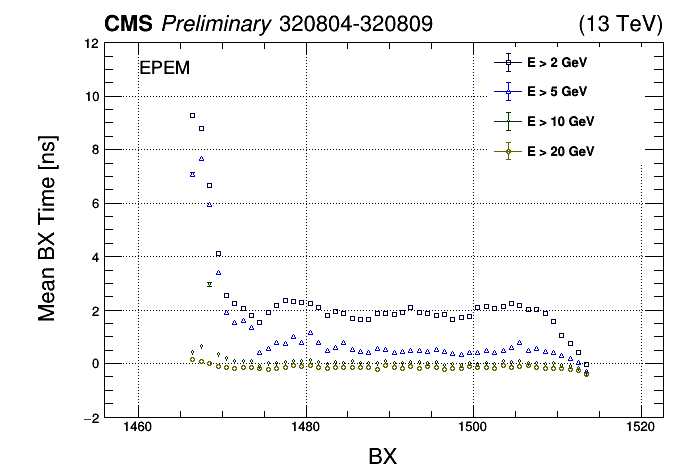
\includegraphics{fig/sec_motive/tr_lhc_18A_ratioall_note_05112021123825.png}}
\caption{The energy dependence of the rechit time on the position of a BX in a train of filled buckets. The mean of all the rechit times for all rechits with specified minimum energy in a single BX are plotted with respect to the BX position of that BX. The effect of OOT pileup on the mean rechit time is shown to be strongly dependent on the rechit energy.}
\label{trianedep}
\end{center}
\end{figure}
 
The impact of empty BXs on he rechit times is explained by the effect of OOT-PU on the measured pulse in an ECAL crystal, as discussed in \ref{sec:reco1}. When energy from OOT-PU contributes to the measured pulse in a crystal, by creating an additional OOT pulse that is superimposed with the nominal pulse, this will pull the peak of the measured pulse away from the peak of the nominal pulse, resulting in the reconstructed arrival time deviating from the actual arrival time of the nominal pulse. If the OOT pulse occurs after the nominal pulse this will cause the reconstructed time to be shift forward, or later, than the nominal time and to be shifted backward, or earlier, if the OOT pulse occurs before the nominal pulse. This effect is observed in Figure~\ref{tam_timeresBX} in which the mean rechit time in a BX is plotted with respect to the BX position for a single sub-train. The first several BXs in the train, in which the filled BXs predominantly occur after them, have mean times that are later then the majority of the train, and the mean times of the last several BXs have earlier mean times since the majority of filled BXs are before them. 
 
%>>>>>>>> This is explained by the effect of OOT-PU on the measured pulse shape as shown in Figure~\ref{tam_pulsesuper}. 

\begin{figure}[!htbp]
\begin{center}
\resizebox{0.7\linewidth}{!}{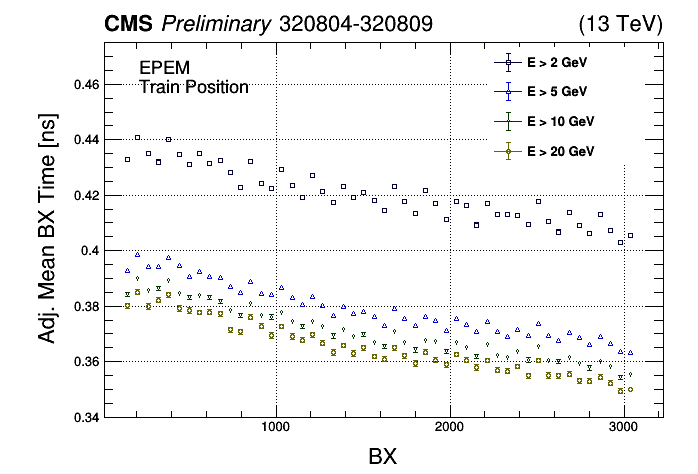
\includegraphics{fig/sec_motive/tr_lhc_18A_ratioall_stp_note_23112021155939.png}}
\caption{The energy dependence of the mean rechit time by BX is shown for all BX positions. The BX positions are grouped in bins of 50 BXs to better resolve the effects at this scale. The mean time is also seen to have an overall dependence on the BX position in the beam cycle. This dependence on BX position was attributed to the drift in the RF phase during the beam cycle.}
\label{tam_timeresbxe}
\end{center}
\end{figure}

%The dependence of the mean rechit time with respect to the BX position for a single sub-train on the rechit energy, $E_{ECAL}$ is seen in Figure~\ref{trianedep}. The mean rechit time for rechits that have $E_{ECAL}$ greater than a specified threshold as shown is plotted with respect to the BX position. There is a marked dependence on $E_{ECAL}$ observed in the mean time which is much stronger in lower energies. The effect of OOT-PU shifts the mean times and degrades the time resolution.

It can also be seen that the rechit time is strongly dependent on the rechit energy, as well as the BX position in a sub-train, in Figure~\ref{trianedep}. The mean rechit time for rechits that have rechit energy greater than the specified thresholds are plotted with respect to the BX position. There is a marked dependence on energy observed in the mean time as this dependence is much stronger at lower energies where the effect of OOT-PU would be expected to have a greater impact.
%The effect of OOT-PU shifts the mean times and degrades the time resolution. 

\begin{figure}[htbp]
\begin{center}
%\resizebox{0.48\linewidth}{!}{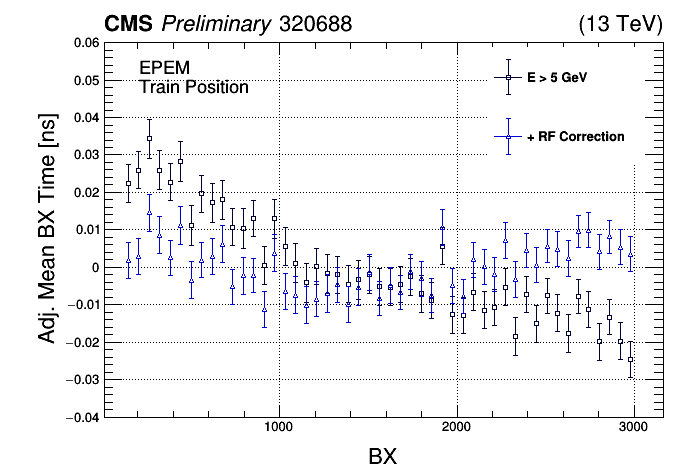
\includegraphics{fig/sec_motive/tr_lhc_18A_rfc_stp_note_23112021145355.png}}
\resizebox{0.7\linewidth}{!}{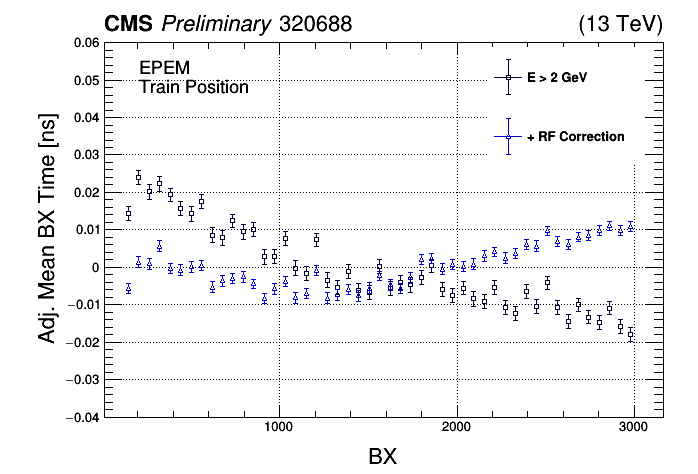
\includegraphics{fig/sec_motive/tr_lhc_18A_rfc_stp_note_23112021150000.png}}
\caption{ The mean rechit time of all rechits in the BXs of a train of filled buckets in which the mean rechit times for all rechits with an energy greater than 2 GeV, adjusted so that the mean rechit time by BX when averaged over all BX positions is zero, as a function of the position of the train in the beam cycle. The first set of data points (squares) shows the dependence of the rechit time on the RF phase drift during the beam cycle. The RF phase corrected data points (triangles) have a correction for the RF Phase drift applied in the time reconstruction. The RF phase correction is shown to have a negligible impact on the time reconstruction.}
\label{tam_lhcrhphasecor}
\end{center}
\end{figure}

In Figure~\ref{tam_timeresbxe} the energy dependence of the mean rechit time by BX is shown for all BX positions. The BX position is grouped in bins of 50 BXs in order to better resolve effects at this scale. Once more the strong dependence of the mean time on the energy is observed. The mean time is also seen to have an overall dependence on the BX position. This dependence on BX position was attributed to the drift in the RF phase during the beam cycle. To account for this dependence on the RF phase, a correction was derived from the RF phase information in LHCInfo. As can be seen in Figure~\ref{tam_lhcrhphasecor}, this correction removes the dependence on the RF cavity frequency, but the effect was negligible compared to issues arising from the OOT-PU dependence.

%\begin{figure}[htbp]
%\begin{center}
%\resizebox{0.42\linewidth}{!}{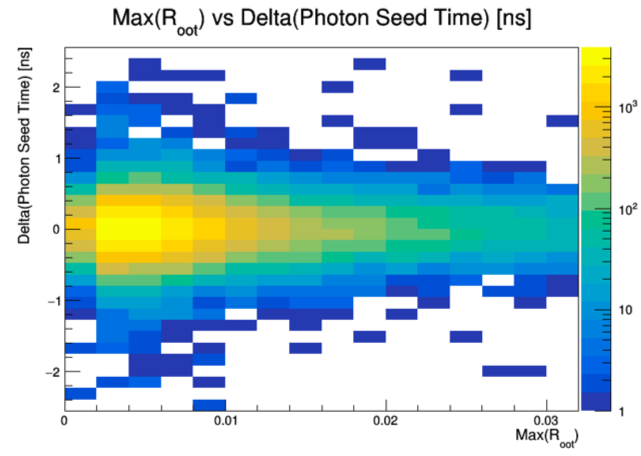
\includegraphics{fig/sec_motive/maxroot_v_photime.png}}
%\caption{The difference in rechit time, or $\Delta(Photon Seed time)$, with respect to Max$(R_{oot})$ as used in the time resolution is plotted. Here we can clearly observe a dependence on the resolution with Max$(R_{oot})$. }
%\label{tam_ootampdtVmax}
%\end{center}
%\end{figure}

Utilizing the information available in the RAW data streams, it is possible to study the ten sampled amplitudes of the measured pulse used to reconstruct the time and energy of a pulse in an ECAL crystal, and thus the time and energy of an reconstructed EG candidate. In the following discussion, "nominal amplitude" will refer to the sampled amplitude which occurs at the nominal time of the BX. Sample amplitudes before and after the nominal amplitude are referred to as OOT amplitudes. OOT pulses that contribute to the measured pulse will have a maximum contribution to the amplitudes of the OOT amplitudes since these contributions are displaced in time from the nominal amplitude. Thus by studying cases when the maximum amplitude occurs before, after or at the nominal amplitude we can see the effect of OOT-PU on the reconstructed times of EG candidates. 

\hfill
\begin{figure}[htbp]
\begin{center}
\resizebox{0.32\linewidth}{!}{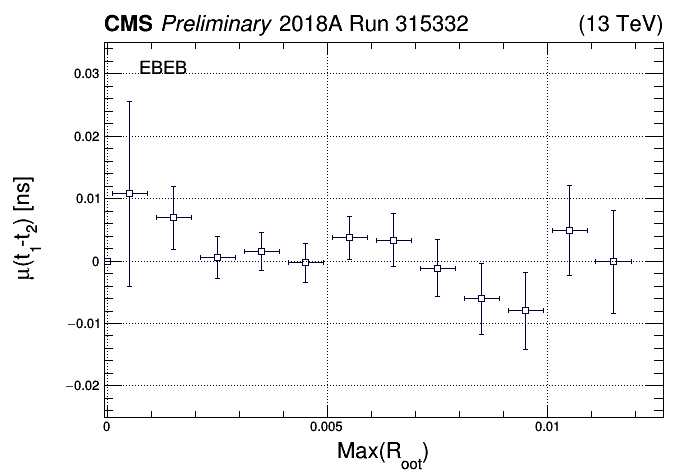
\includegraphics{fig/sec_motive/tr_hl_ootAmpMax_mean_17112021154025.png}}
\resizebox{0.32\linewidth}{!}{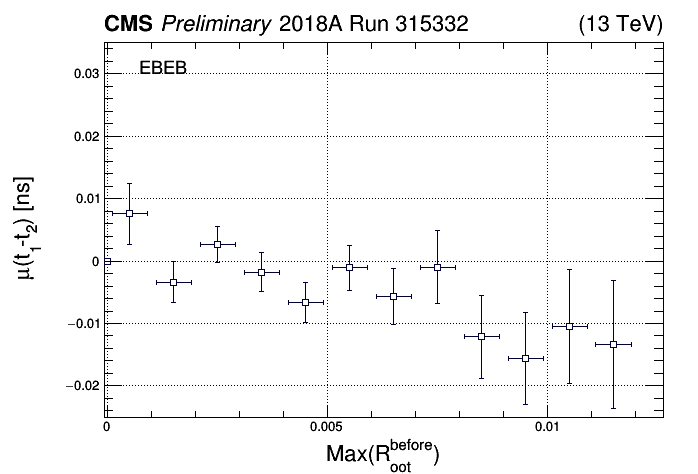
\includegraphics{fig/sec_motive/tr_hl_ootAmpMBfr_mean_17112021155948.png}}
\resizebox{0.32\linewidth}{!}{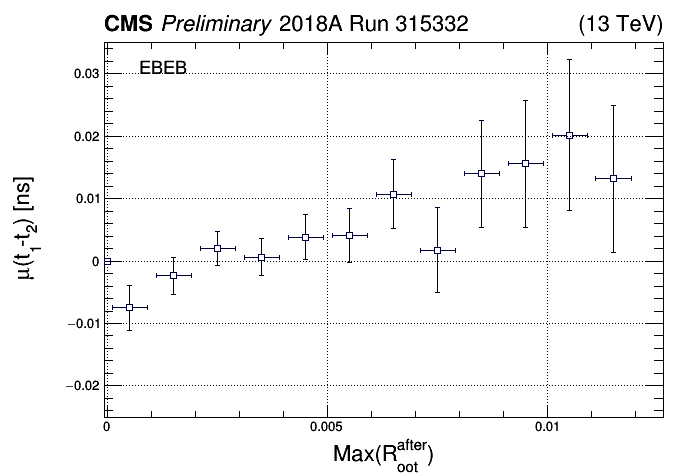
\includegraphics{fig/sec_motive/tr_hl_ootAmpMAft_mean_17112021155914.png}}
\resizebox{0.32\linewidth}{!}{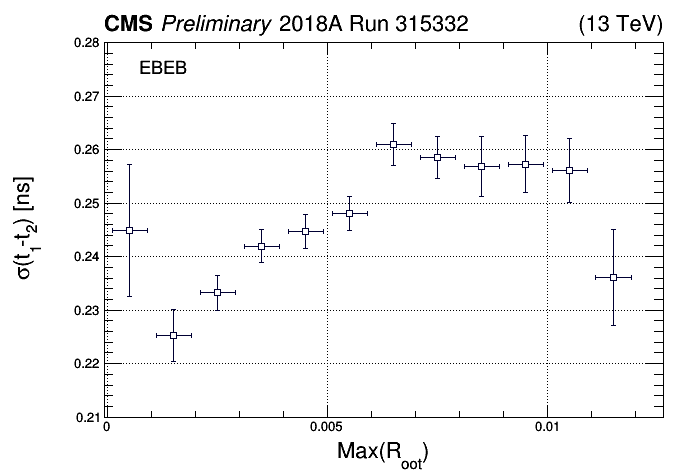
\includegraphics{fig/sec_motive/tr_hl_ootAmpMax_sigma_17112021150325.png}}
\resizebox{0.32\linewidth}{!}{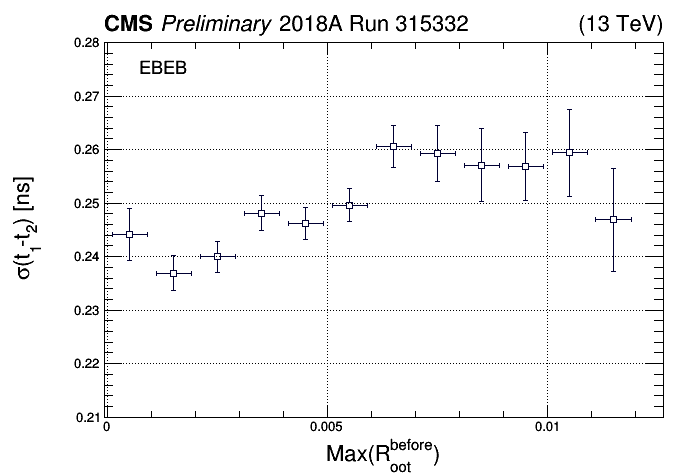
\includegraphics{fig/sec_motive/tr_hl_ootAmpMBfr_sigma_17112021151827.png}}
\resizebox{0.32\linewidth}{!}{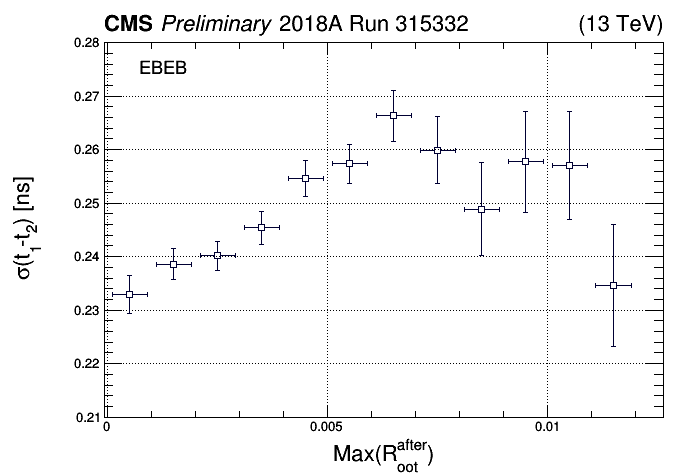
\includegraphics{fig/sec_motive/tr_hl_ootAmpMAft_sigma_17112021151937.png}}
\caption{Mean ($\mu$, top) and width ($\sigma$, bottom) of the difference in the reconstructed times for the seed crystal of an EG candidate and an adjacent crystal to the seed crystal are shown as a function of the three cases of the ratio, $R_{oot}$, of the nominal amplitude to the maximum OOT amplitude. Max$(R_{oot})$, the largest ratio found amongst all nine of the OOT amplitudes, is shown on the left. Max$(R_{oot}^{before})$, the largest ratio found amongst the five OOT amplitudes before the nominal amplitude, is shown in the middle. And Max$(R_{oot}^{after})$, the largest ratio found amongst the four OOT amplitudes after the nominal amplitude, is shown on the right. The plots for $\mu$ indicate that the mean of the time difference is biased in the direction of the larger values of $R_{oot}$. The plots for $\sigma$ indicate that in all cases the width of the distribution increases with larger values of $R_{oot}$.}
\label{tam_ootampbias}
\end{center}
\end{figure}

The ratio of the nominal amplitude to the maximum OOT amplitude, $R_{oot}$, from all nine OOT amplitudes, the ratio of the nominal amplitude to the maximum OOT amplitude that occurred in the five BXs before the nominal amplitude, $R_{oot}^{before}$, and the ratio of the maximum OOT amplitude that occurred in the four BXs after the nominal amplitude, $R_{oot}^{after}$ were studied. Larger values of these ratios will indicate a significant contribution in the measured amplitudes from OOT pile-up in the event. In order to examine the effect on the time reconstruction, the seed crystal of an EG candidate and an adjacent crystal to the seed crystal are selected. From the two sets of amplitudes in the adjacent crystals the maximum value of $R_{oot}$ ($R_{oot}^{before}$, $R_{oot}^{after}$), Max$(R_{oot})$ (Max$(R_{oot}^{before})$, Max$(R_{oot}^{after})$) and the difference in the reconstructed times of the measured pulse of in the crystals, $\Delta(Photon Seed time)$, was determined. The mean ($\mu$), and width ($\sigma$) of the distribution of $\Delta(Photon Seed time)$ in bins of Max$(R_{oot})$ (Max$(R_{oot}^{before})$, Max$(R_{oot}^{after})$) was determined.

In Figure~\ref{tam_ootampbias} the $\mu$, top, and $\sigma$, bottom, of $\Delta(Photon Seed time)$ is shown as a function of; Max$(R_{oot})$, right; Max$(R_{oot}^{before})$, center;  and Max$(R_{oot}^{after})$, left. As seen in the plots on the left, for the Max$(R_{oot})$, $\mu$ is consistent with the expected value of zero while $\sigma$ degrades with large values of Max$(R_{oot})$. For Max$(R_{oot}^{before})$ the $\mu$ is shifted negative, or back in time, as the magnitude of OOT amplitudes occurring before the nominal amplitude increases. In the plots for the Max$(R_{oot}^{after})$ we see the same effect on the $\mu$ but in the opposite direction, as expected if the magnitude of OOT amplitudes occurring after the nominal amplitude increases. These results are both consistent with our understanding of the effect of OOT amplitudes on the measured pulse shape as discussed previously. In all cases Figure~\ref{tam_ootampbias} shows that the $\sigma$ is degraded by $\sim$30 ps. The contribution of the OOT-PU to this observed degradation is in quadrature with other contributions and on the order of 100 ps.

%Determine the BX position  allows us to do this.
%We utilized the RF data in LHCInfo to calculate a phase correction to the nominal collision time of the proton packets in a BX

%\begin{figure}[htbp]
%\begin{center}
%\resizebox{0.42\linewidth}{!}{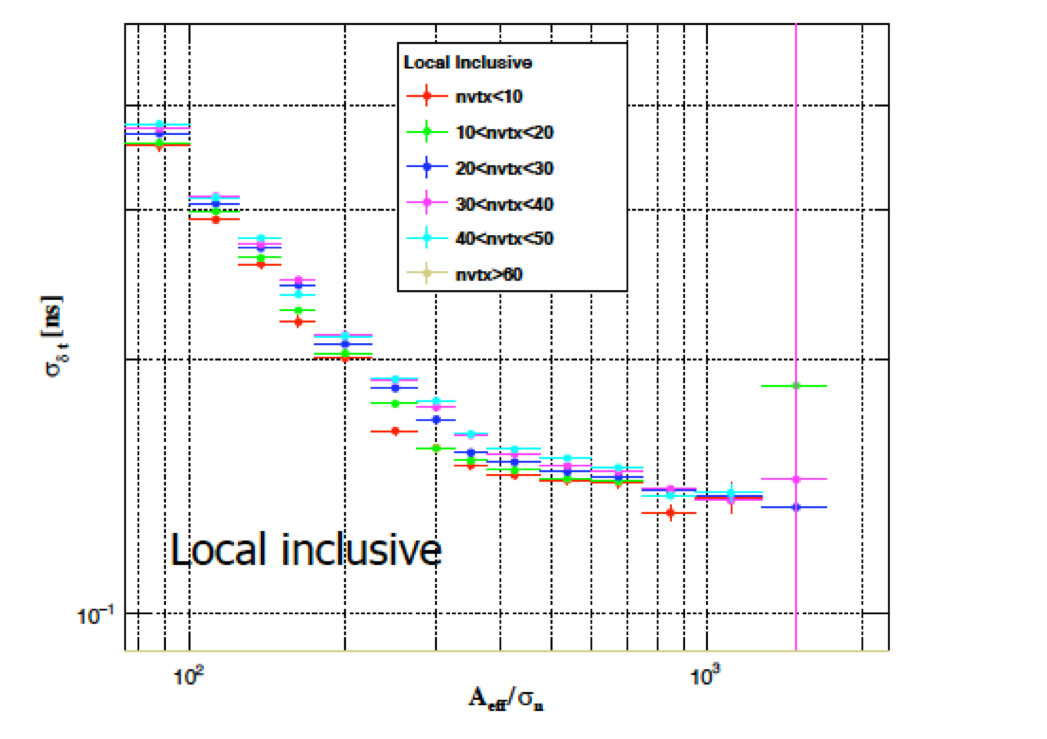
\includegraphics{fig/sec_motive/timeres_v_nvtx2017.png}}
%\caption{$Local Inclusive$ resolutions for a portion of the Run2018 EGamma miniAOD stream comparing the resolution in categories determined by the number of vertexes in each event. In this plot we see that as the number of vertexes increases, and the resolution degrades and the amount of OOT pile-up increases.
%}
%\label{tam_timeresnvtx}
%\end{center}
%\end{figure}

%These three cases are shown in Figure~\ref{tam_ootampdtVmax}

%of the ratio of the OOT amplitudes to the nominal amplitude where studied in Figure~\ref{tam_ootampdtVmax}. Figure~\ref{tam_ootampdtVmax} shows the distribution of difference of the rechit times in the crystal pairs with respect to Max$(R_{oot})$. The width of the distribution of the difference in rechit times gives a time resolution in bins of Max$(R_{oot})$. It can be seen that resolution degrades significantly when there is larger amounts of OOT pile-up present in the event as indicated by larger values of Max$(R_{oot})$.
%Cases where the largest OOT amplitude occurs before and after the nominal BX to determine the effect of location of the largest OOT amplitude on the time reconstruction. 
%Plots for both the mean time difference, $\mu$ on the top row and the time resolution, $\sigma$ on the bottom row, are shown in all three cases. 